%%%%%%%%%%%%%%%%%%%%%%%%%%%%%%%%%%%%%%%%%%%%%%%%%%%%%%
%%%%%%%%%%%%%%%%%%%%%%%%%%%%%%%%%%%%%%%%%%%%%%%%%%%%%%
\section[Model based optim.]{Model based optimization methods}
\subsection{}

%%%%%%%%%%%%%%%%%%%%%%%%%%%%%%%%%%%%%%%%%%%%%%%%%%%%%%
\begin{frame}{}
If the number of function evaluations are limited, we can run the optimization on the model instead of running it directly on the function
\begin{center}
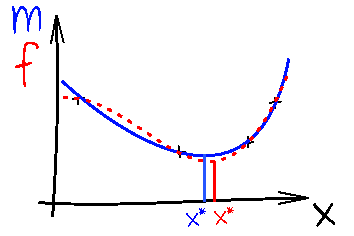
\includegraphics[height=5cm]{4_optimization/figures/ink_mf}
\end{center}
In the end, we hope that:
\begin{equation*}
	\begin{split}
		\argmin(m) & \approx \argmin(f)\\
		\min(m) & \approx \min(f)\\
	\end{split}
\end{equation*}
\end{frame}

%%%%%%%%%%%%%%%%%%%%%%%%%%%%%%%%%%%%%%%%%%%%%%%%%%%%%%
\begin{frame}{}
\structure{Overall framework}
  \begin{figure}
    \centering \sf
    \begin{tikzpicture}[scale=0.7, every node/.style={scale=0.6}]

      % \tikzstyle{Sim}=[rectangle, draw=MonBleu!20, fill=MonBleu!0];
      % \tikzstyle{Meta}=[rectangle, draw=Orange!40, fill=MonBleu!0];
      \tikzstyle{Mes}=[rectangle, draw=violet!20, fill=violet!0];

        \node[Mes](MesIn) at (-6, 0) {
          \parbox{2.2cm}{ %
            \centering
            \LARGE
            \vspace{3mm}
            $x$
            \vspace{3mm}
          }};

        \node[Mes](Mes) at (0, 0) {
          \parbox{4.5cm}{ %
            \centering
            \LARGE
            \vspace{4mm}
            \textit{costly function}\\
            \vspace{4mm}
          }};

        \node[Mes](MesOut) at (6, 0) {
        \parbox{4.5cm}{ %
            \centering
            \LARGE
            \vspace{3mm}
          \textit{observations}\\
            \vspace{3mm}
        }};
        \draw[->, very thick, draw=MonBleu] (MesIn) -- (Mes.west);
        \draw[->, very thick, draw=MonBleu] (Mes) -- (MesOut.west);

        \node[Mes](MetaIn) at (-6, -4.5) {
          \parbox{2.2cm}{ %
          \centering
            \LARGE
            \vspace{3mm}
            $x$
            \vspace{3mm}
          }};

        \node[Mes](Meta) at (0, -4.5) {
          \parbox{4.5cm}{ %
            \centering
            \LARGE
            \vspace{4mm}
            \textit{surrogate model}\\
            \vspace{4mm}
          }};

        \node[Mes](MetaOut) at (6.0, -4.5) {
        \parbox{4.5cm}{ %
            \centering
            \LARGE
            \vspace{3mm}
          \textit{approximations}\\
            \vspace{3mm}
        }};

        \draw[->, very thick, draw=MonBleu] (MetaIn) -- (Meta.west);
        \draw[->, very thick, draw=MonBleu] (Meta) -- (MetaOut.west);

        \draw[->, very thick, draw=Orange!80] (MesIn) -- (Meta)
        node [above, midway, sloped, Orange!80] {\large Design of Experiments};
        \draw[->, very thick, draw=Orange!80] (MesOut)  -- (Meta);
        %node [above, midway, sloped, Orange!80] {\large réponses};

    \end{tikzpicture}
    \end{figure}
In practice, it is risky to take decisions based only on the model...\\
\vspace{3mm}
On the other hand, the model can be used to guide us in the search for the optimum.
\end{frame}

%%%%%%%%%%%%%%%%%%%%%%%%%%%%%%%%%%%%%%%%%%%%%%%%%%%%%%
\begin{frame}{}
Global optimization methods are a trade-off between
\begin{itemize}
	\item Exploitations of good results
	\item Exploration of the space
\end{itemize}
\vspace{3mm}
\begin{center}
\textbf{How can GPR models be helpful?}\\
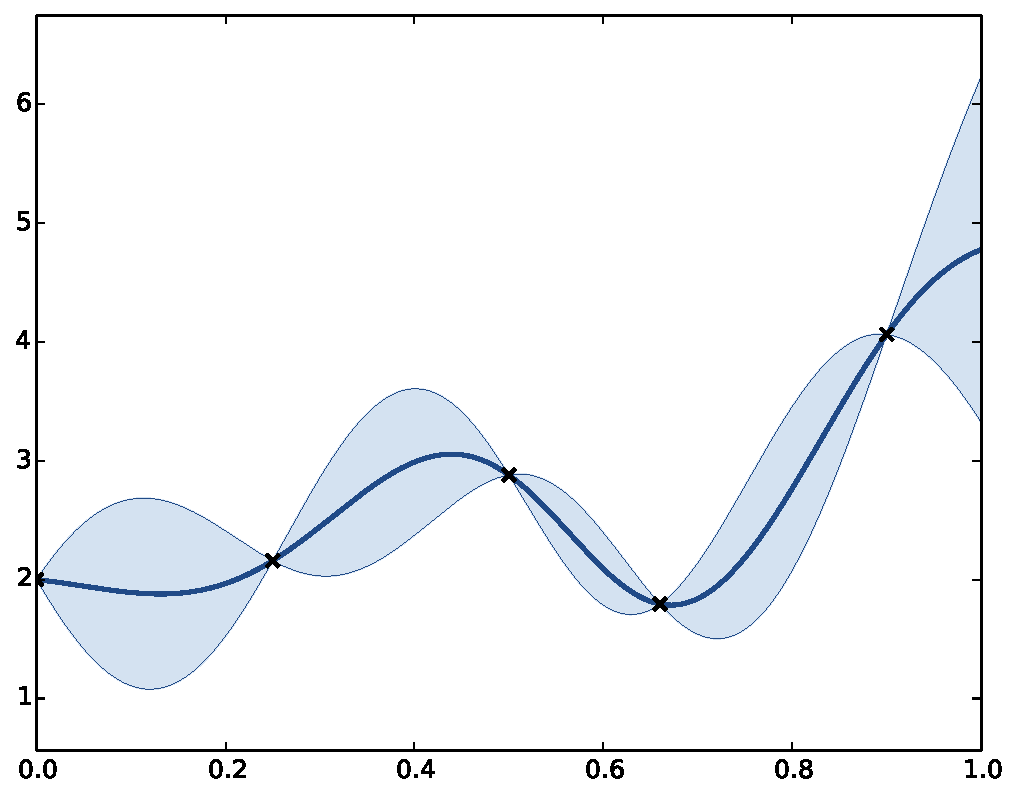
\includegraphics[height=5cm]{4_optimization/figures/python/ego_0}
\end{center}
\end{frame}

%%%%%%%%%%%%%%%%%%%%%%%%%%%%%%%%%%%%%%%%%%%%%%%%%%%%%%
\begin{frame}{}
In our example, the best observed value is 1.79
\begin{center}
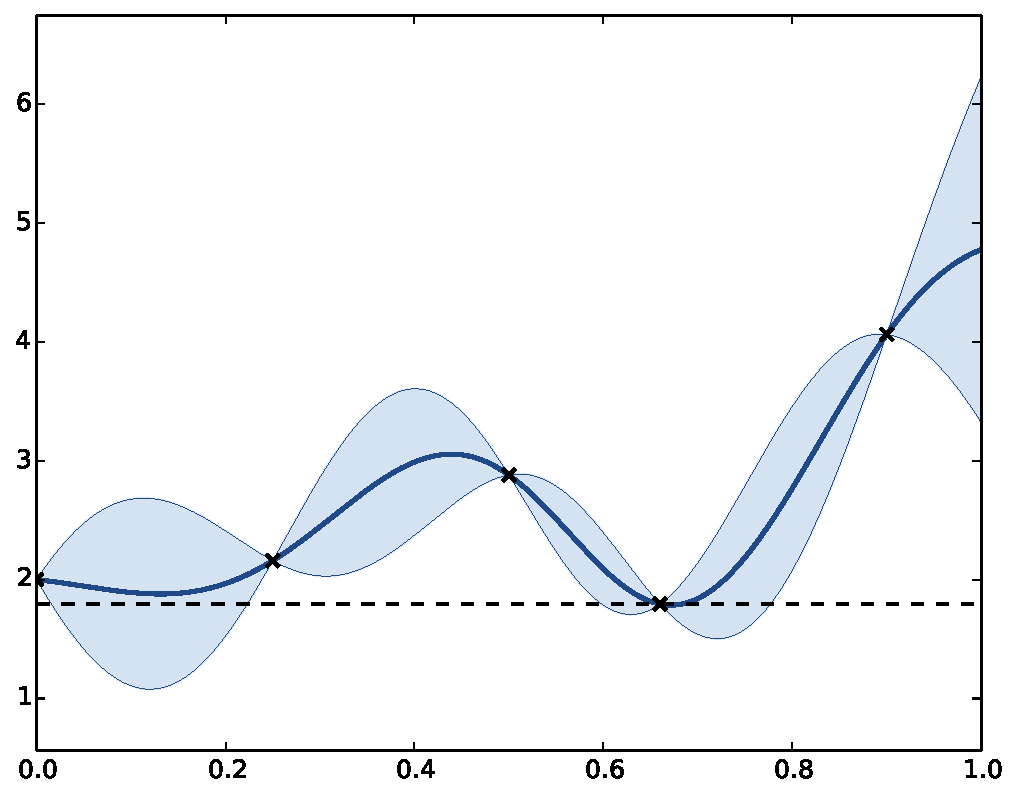
\includegraphics[height=5cm]{4_optimization/figures/python/ego_improv}
\end{center}
Various criteria can be studied
\begin{itemize}
	\item probability of improvement
	\item Expected improvement
\end{itemize}
\end{frame}

%%%%%%%%%%%%%%%%%%%%%%%%%%%%%%%%%%%%%%%%%%%%%%%%%%%%%%
\begin{frame}{}
\textbf{Probability of Improvement:}
$$PI(x) = cdf \left(\frac{\min(F) - m(x)}{\sqrt{(c(x,x))}} \right)$$
\begin{center}
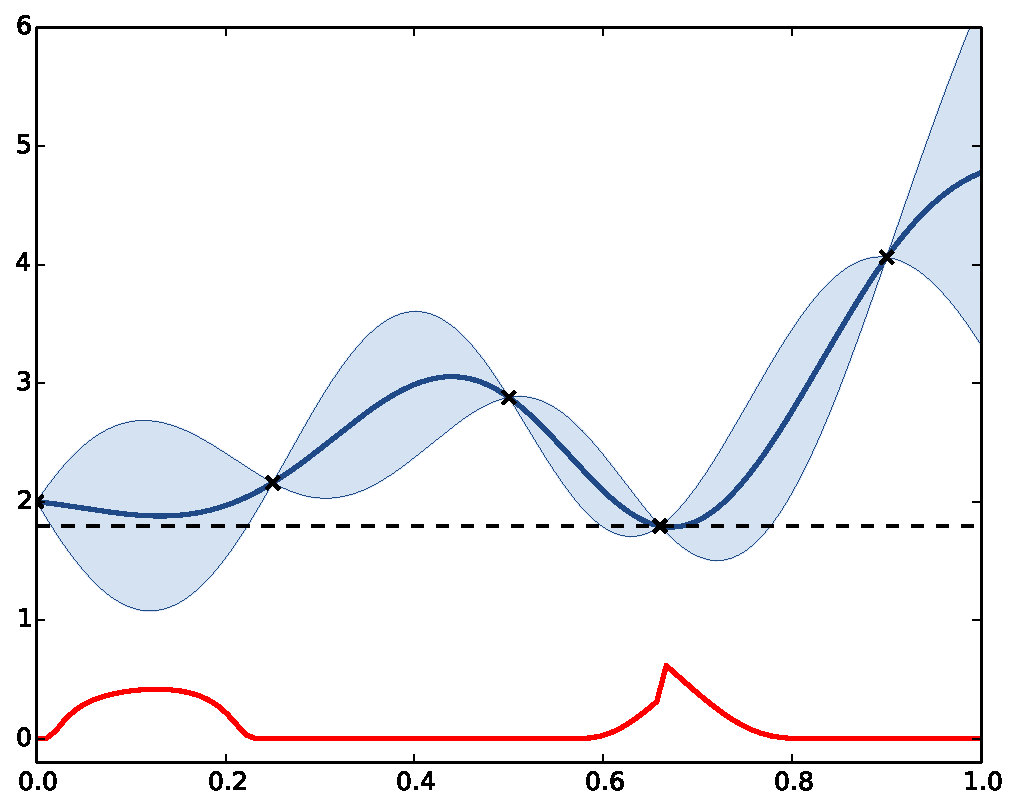
\includegraphics[height=5cm]{4_optimization/figures/python/ego_PI}
\end{center}
\end{frame}

%%%%%%%%%%%%%%%%%%%%%%%%%%%%%%%%%%%%%%%%%%%%%%%%%%%%%%
\begin{frame}{}
The point with the highest PI is often very close to the best observed value. We can show that there is a $x$ in the neighbourhood of $x^*$ such that $PI(x) \geq 0.5$.\\
\vspace{5mm}
For such points, the improvement cannot be large... \\
\vspace{3mm}
Can we find another criterion?
\end{frame}

%%%%%%%%%%%%%%%%%%%%%%%%%%%%%%%%%%%%%%%%%%%%%%%%%%%%%%
\begin{frame}{}
\textbf{Expected Improvement:}
$$EI(x) = \sqrt{c(x,x)} (u(x) cdf(u(x)) + pdf(u(x)))$$
\qquad with $ \displaystyle u(x) = \frac{\min(F) - m(x)}{\sqrt{(c(x,x))}}$
\begin{center}
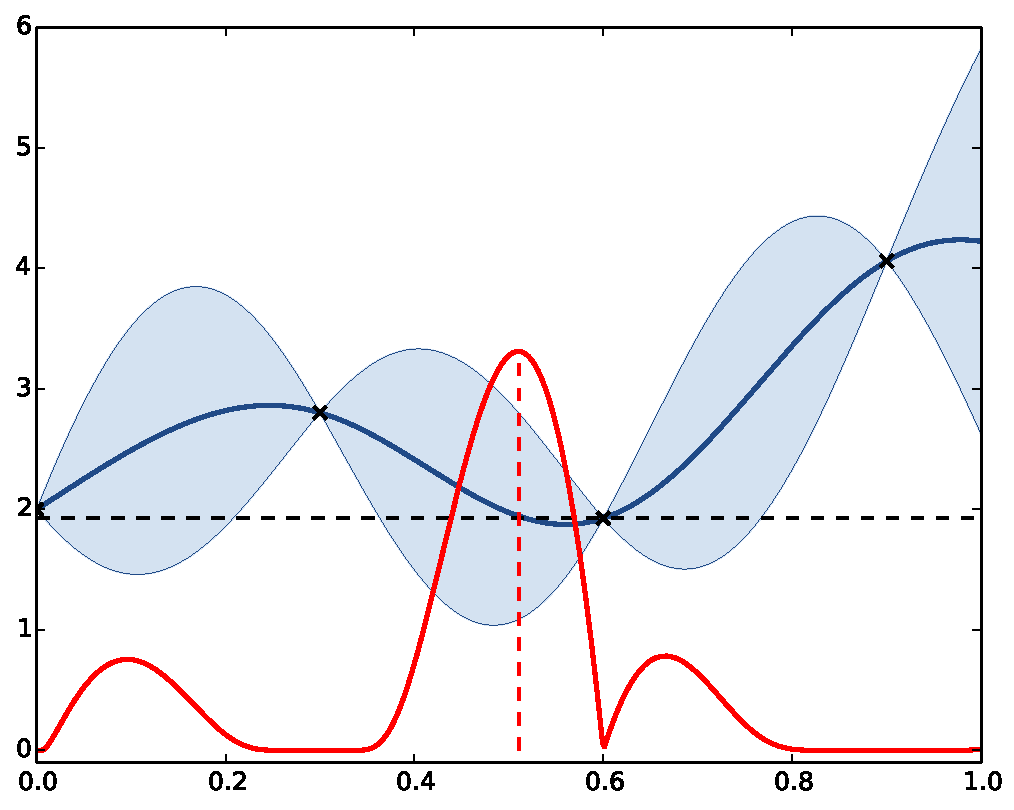
\includegraphics[height=5cm]{4_optimization/figures/python/ego_EI0}
\end{center}
\end{frame}

%%%%%%%%%%%%%%%%%%%%%%%%%%%%%%%%%%%%%%%%%%%%%%%%%%%%%%
\begin{frame}{Expected Improvement}
Let's see how it works... iteration 1
\begin{center}
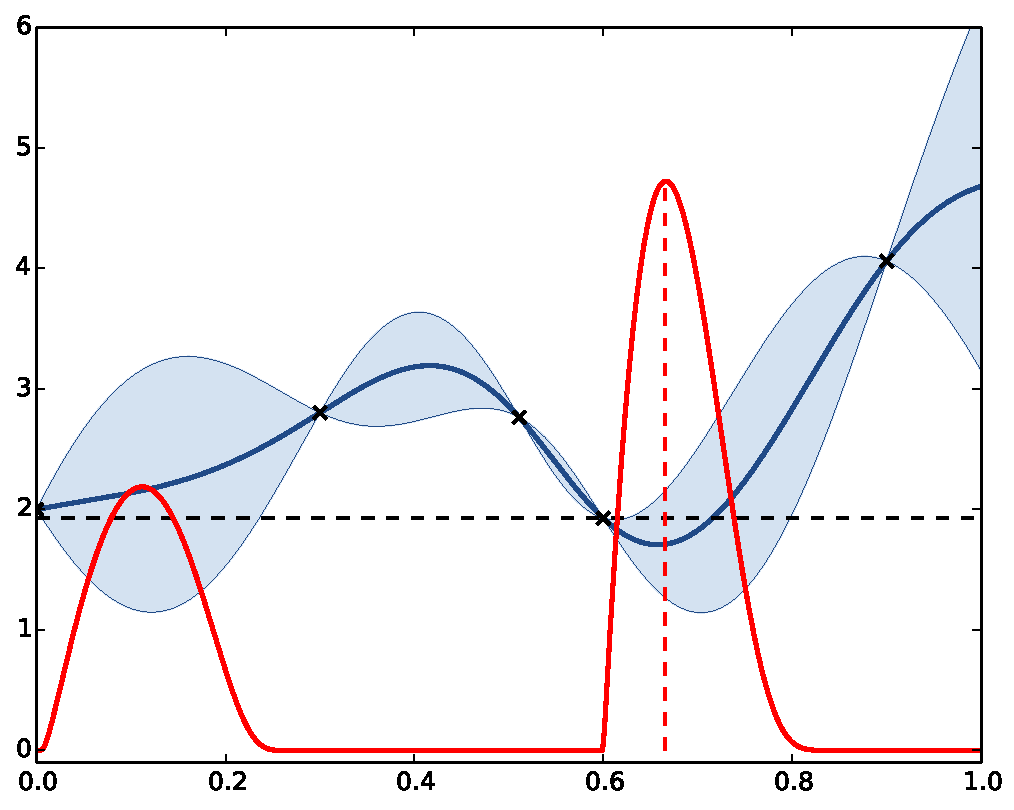
\includegraphics[height=5cm]{4_optimization/figures/python/ego_EI1}
\end{center}
\end{frame}

%%%%%%%%%%%%%%%%%%%%%%%%%%%%%%%%%%%%%%%%%%%%%%%%%%%%%%
\begin{frame}[noframenumbering]{Expected Improvement}
Let's see how it works... iteration 2
\begin{center}
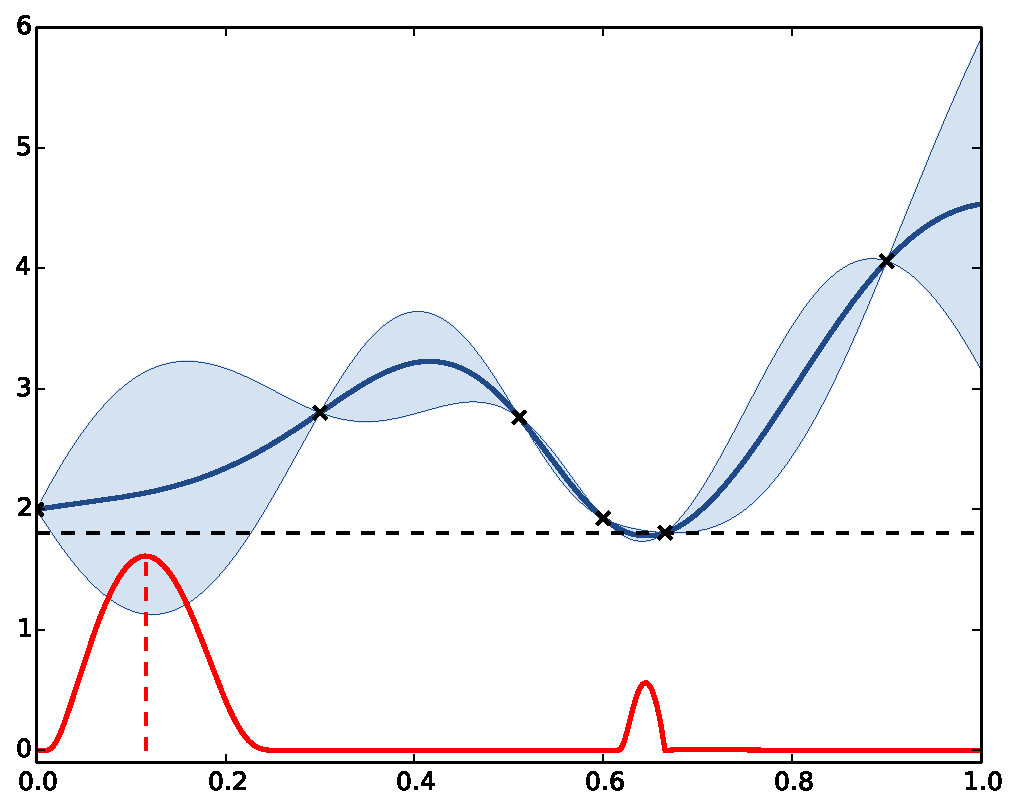
\includegraphics[height=5cm]{4_optimization/figures/python/ego_EI2}
\end{center}
\end{frame}

%%%%%%%%%%%%%%%%%%%%%%%%%%%%%%%%%%%%%%%%%%%%%%%%%%%%%%
\begin{frame}[noframenumbering]{Expected Improvement}
Let's see how it works... iteration 3
\begin{center}
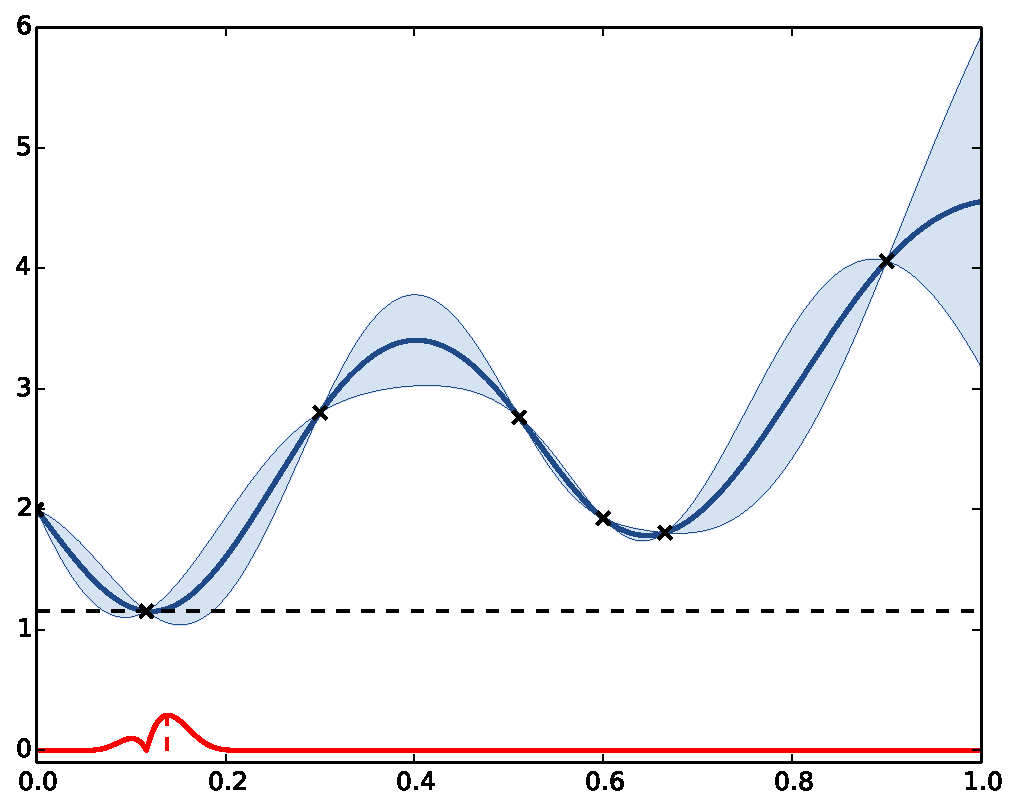
\includegraphics[height=5cm]{4_optimization/figures/python/ego_EI3}
\end{center}
\end{frame}

%%%%%%%%%%%%%%%%%%%%%%%%%%%%%%%%%%%%%%%%%%%%%%%%%%%%%%
\begin{frame}[noframenumbering]{Expected Improvement}
Let's see how it works... iteration 4
\begin{center}
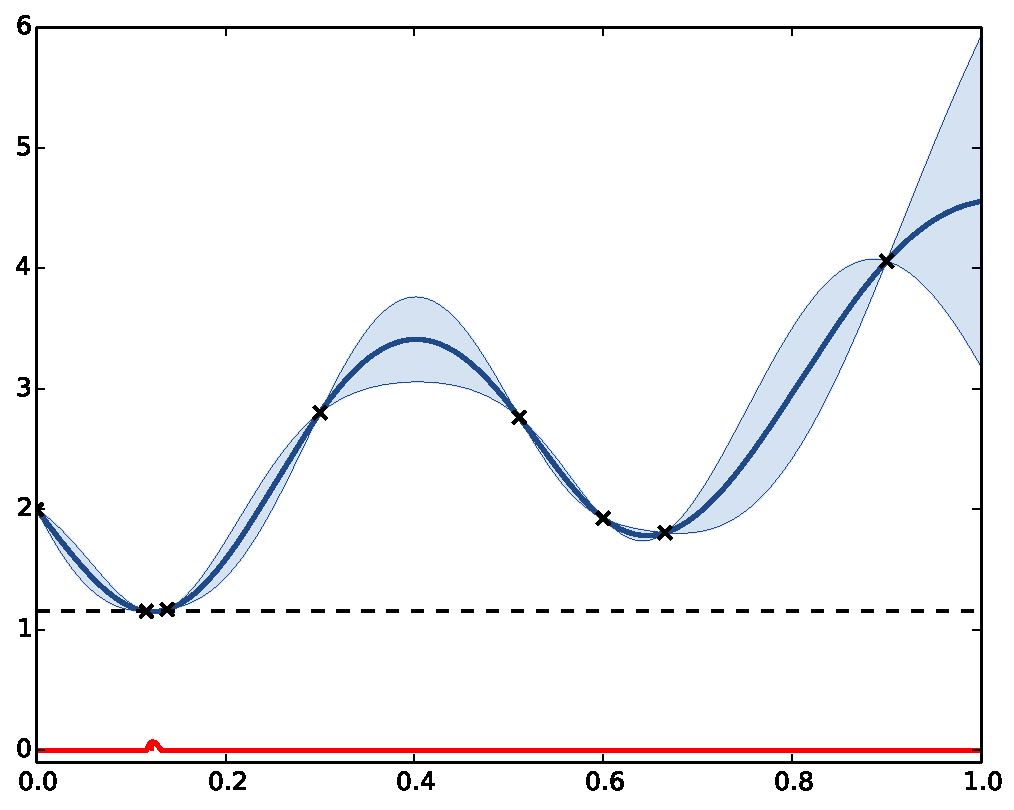
\includegraphics[height=5cm]{4_optimization/figures/python/ego_EI4}
\end{center}
\end{frame}

%%%%%%%%%%%%%%%%%%%%%%%%%%%%%%%%%%%%%%%%%%%%%%%%%%%%%%
\begin{frame}[noframenumbering]{Expected Improvement}
Let's see how it works... iteration 5
\begin{center}
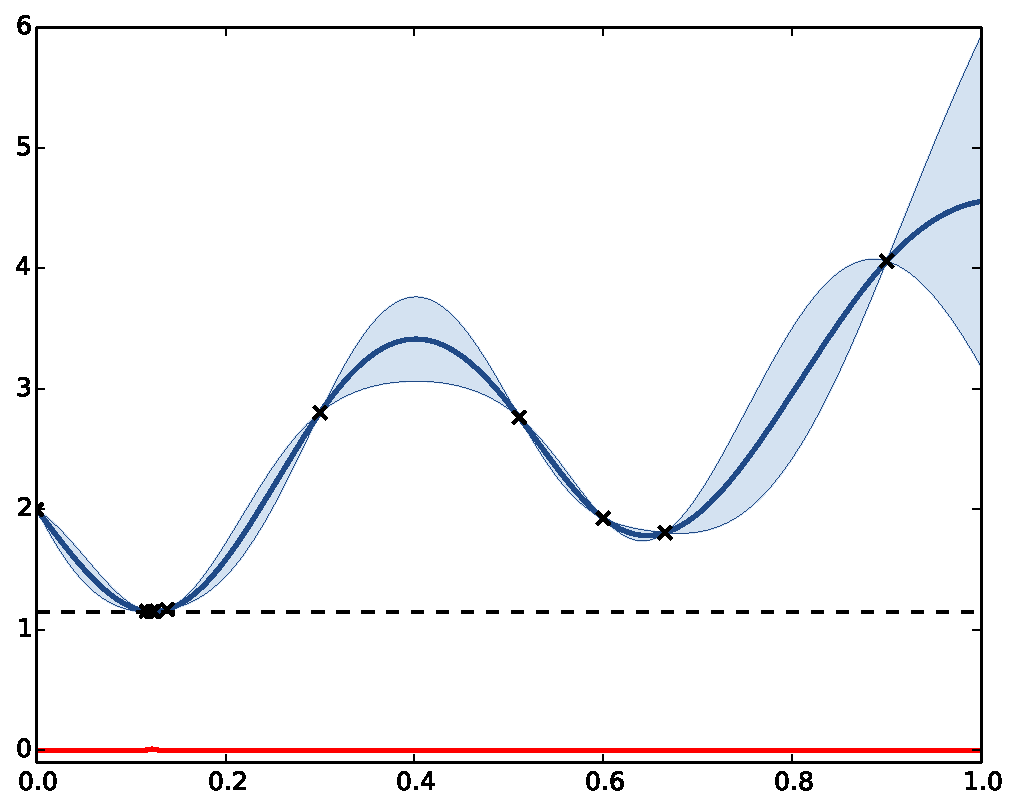
\includegraphics[height=5cm]{4_optimization/figures/python/ego_EI9}
\end{center}
\end{frame}

%%%%%%%%%%%%%%%%%%%%%%%%%%%%%%%%%%%%%%%%%%%%%%%%%%%%%%
\begin{frame}{}

\begin{exampleblock}{Illustration for $d=6$ (Hartman)}
	Illustration in higher dimension
\begin{center}
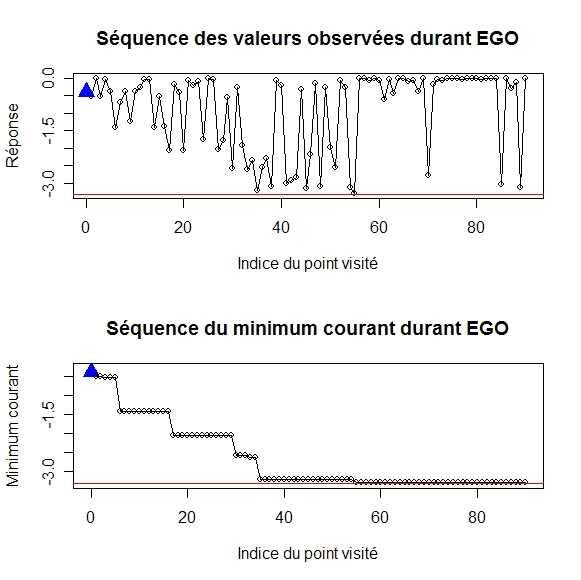
\includegraphics[height=5.5cm]{4_optimization/figures/egoHartman} 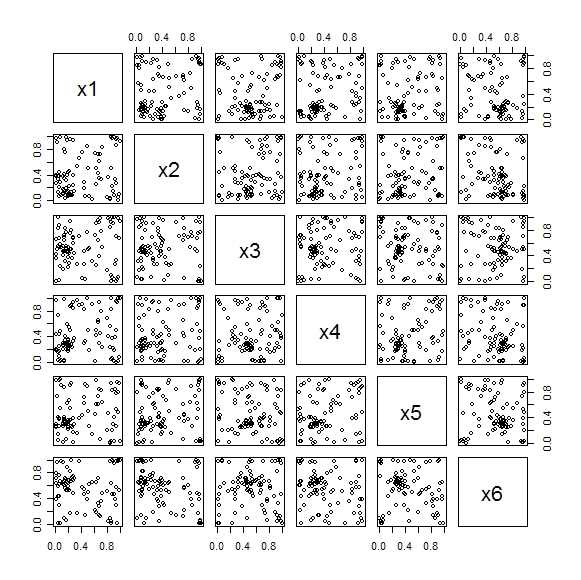
\includegraphics[height=5.5cm]{4_optimization/figures/egoHartman2}
\end{center}
\small Source: DiceOptim, D. Ginsbourger, 2009.
\end{exampleblock}
\end{frame}

%%%%%%%%%%%%%%%%%%%%%%%%%%%%%%%%%%%%%%%%%%%%%%%%%%%%%%
\begin{frame}{Expected Improvement}
This algorithm is called \textbf{Efficient Global Optimization} (EGO). It is famous since a paper of Jones et Al in 1998.\\
\vspace{5mm}
\begin{itemize}
	\item[+] EGO provides a good trade-off between exploitation and exploration.
	\item[+] It only requires a few function observations (10 in the example)
\end{itemize}
One issue is that we may have a model with observations very close one from each other\\
\begin{example}
From the previous 5 iterations, we obtain $1.44e39$ for the conditioning of the covariance matrix. Eigenvalues are
$$ (67.70,\  24.86,\  5.13,\  1.68,\  0.45,\  0.16,\  0.01,\  0.00,\  0.00,\ 0.00) $$
\end{example}
\end{frame}

%%%%%%%%%%%%%%%%%%%%%%%%%%%%%%%%%%%%%%%%%%%%%%%%%%%%%%
\begin{frame}{}
One way to improve the conditioning of the covariance matrix is to replace two values that are close-by by one function value and one derivative:
\begin{center}
  \begin{tabular}{ccc}
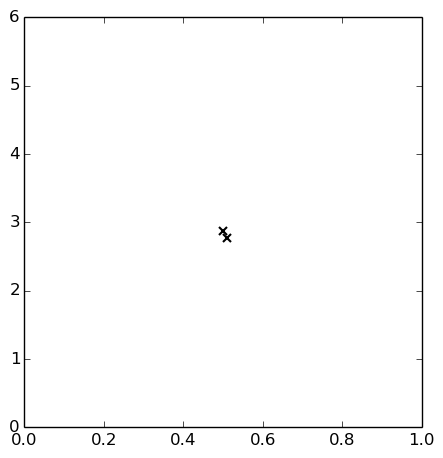
\includegraphics[height=4cm]{4_optimization/figures/python/osborn0} &

\includegraphics[height=4cm]{4_optimization/figures/Rightarrow} &
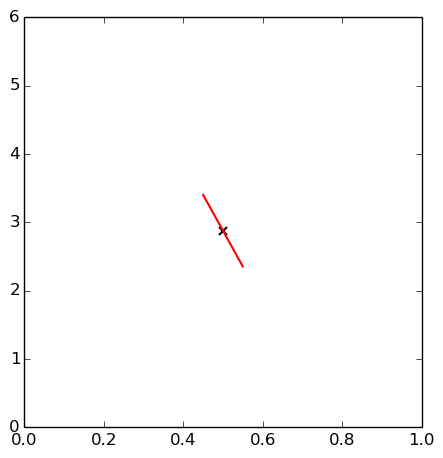
\includegraphics[height=4cm]{4_optimization/figures/python/osborn1} \\
Cond. = 3842 & & Cond. = 10
  \end{tabular}
\end{center}
This can be generalised to higher orders \alert{$\rightarrow$} Taylor expansion\\
\small see articles from M. Osborn
\end{frame}

%%%%%%%%%%%%%%%%%%%%%%%%%%%%%%%%%%%%%%%%%%%%%%%%%%%%%%
\begin{frame}{}
If we know the computational budget in advance, adding new points at the \textbf{best one step ahead location} is not optimal.\\
\vspace{5mm}
Some improvements have been made toward this
\begin{itemize}
	\item Batch EGO
	\item Parallelization of the algorithm
\end{itemize}
\vspace{5mm}
\small see works from D. Ginsbourger
\end{frame}

%%%%%%%%%%%%%%%%%%%%%%%%%%%%%%%%%%%%%%%%%%%%%%%%%%%%%%
%%%%%%%%%%%%%%%%%%%%%%%%%%%%%%%%%%%%%%%%%%%%%%%%%%%%%%
\section[Robust optim.]{Robust optimization}
\subsection{}

%%%%%%%%%%%%%%%%%%%%%%%%%%%%%%%%%%%%%%%%%%%%%%%%%%%%%%
\begin{frame}{}
Robust optimization may mean various things:
\begin{itemize}
	\item There is observation noise on the output
	\item Some input variables are uncertain
	\item Model is uncertain
\end{itemize}
\vspace{2mm}
\begin{example}
\begin{columns}[c]
\column{3cm}
	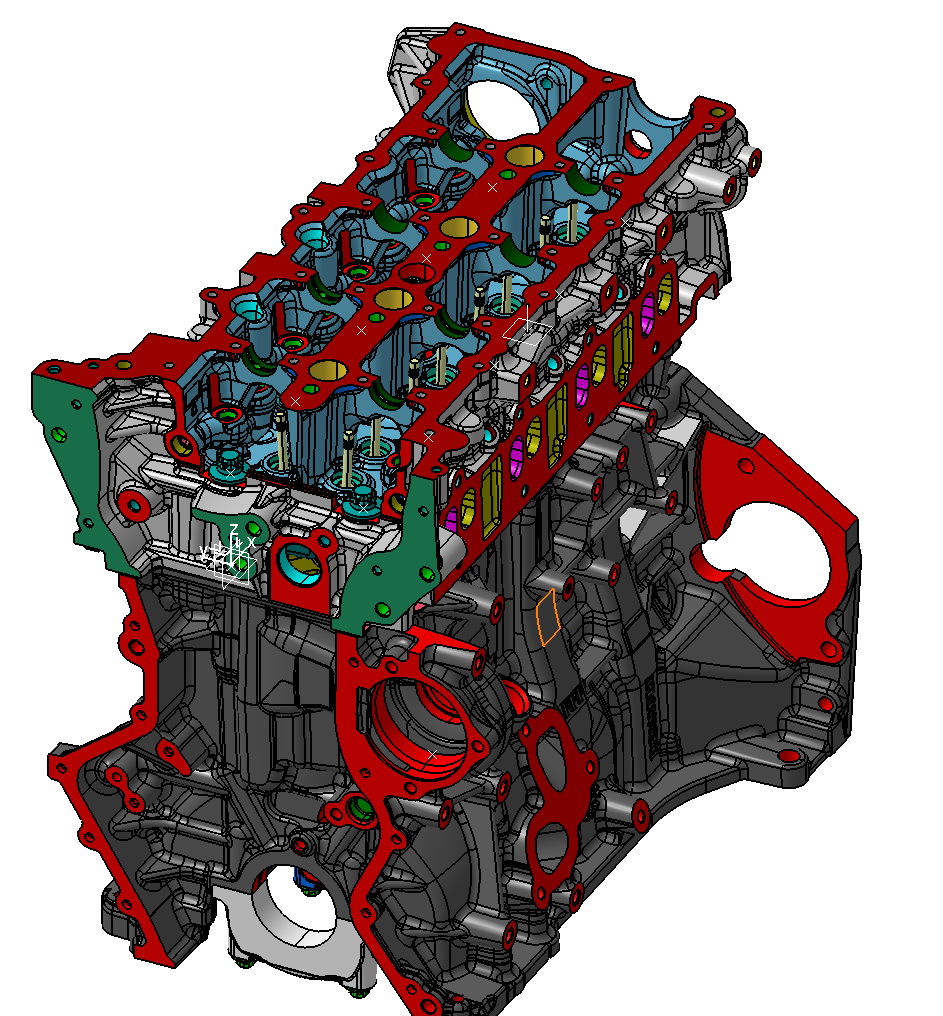
\includegraphics[height=4cm]{4_optimization/figures/RLRrobust}
\column{5cm}
	a +/- 1mm dispersion in the manufacturing of a car cylinder head  can degrade its performance (g CO2/km) by -20\% (worst case)\\
\end{columns}
\vspace{3mm}
	\small Source: Talk from R. Le Riche at the Porquerolles Summer School, 2014
\end{example}
\end{frame}

%%%%%%%%%%%%%%%%%%%%%%%%%%%%%%%%%%%%%%%%%%%%%%%%%%%%%%
\begin{frame}{}
% \begin{example}
% Here is a basic example:
% \begin{center}
% 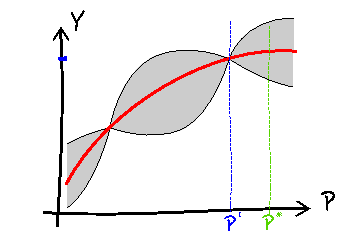
\includegraphics[height=5cm]{4_optimization/figures/optim_rob_a}\\
% Which input is the best?
% \end{center}
% \end{example}
% \end{frame}

% %%%%%%%%%%%%%%%%%%%%%%%%%%%%%%%%%%%%%%%%%%%%%%%%%%%%%%
% \begin{frame}[noframenumbering]{}
\begin{example}
Here is a basic example:
\begin{center}
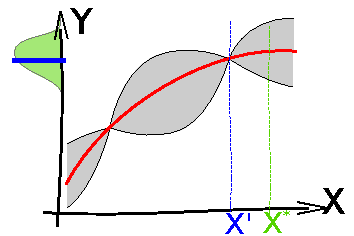
\includegraphics[height=5cm]{4_optimization/figures/optim_rob_b}\\
Which input is the best?
\end{center}
\end{example}
\end{frame}

%%%%%%%%%%%%%%%%%%%%%%%%%%%%%%%%%%%%%%%%%%%%%%%%%%%%%%
\begin{frame}[noframenumbering]{}
\begin{example}
A non Gaussian example
\begin{center}
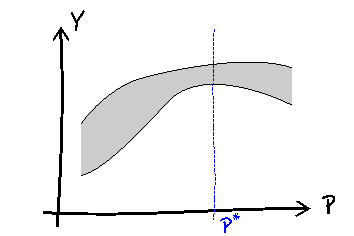
\includegraphics[height=5cm]{4_optimization/figures/optim_rob_c}\\
In some cases, we may want to optimize the worst case scenario.
\end{center}
\end{example}
\end{frame}

%%%%%%%%%%%%%%%%%%%%%%%%%%%%%%%%%%%%%%%%%%%%%%%%%%%%%%
\begin{frame}{}
Can EGO be adapted when observations are noisy?\\
\vspace{5mm}
First of all, using the current best observation as a minimum does not make much sense...\\
\vspace{5mm}
Some solutions are
\begin{itemize}
	\item[S1] Build a new model that interpolates $m(X)$ at $X$.
	\item[S2] Include observation noise and replace $\min(F)$ by $\min(m(X))$ in the EI expression
	\item[S3] Similar to 2 but consider an Expected Mean Improvement.
\end{itemize}
\end{frame}

%%%%%%%%%%%%%%%%%%%%%%%%%%%%%%%%%%%%%%%%%%%%%%%%%%%%%%
\begin{frame}{Solution 1}
iteration 0
\begin{center}
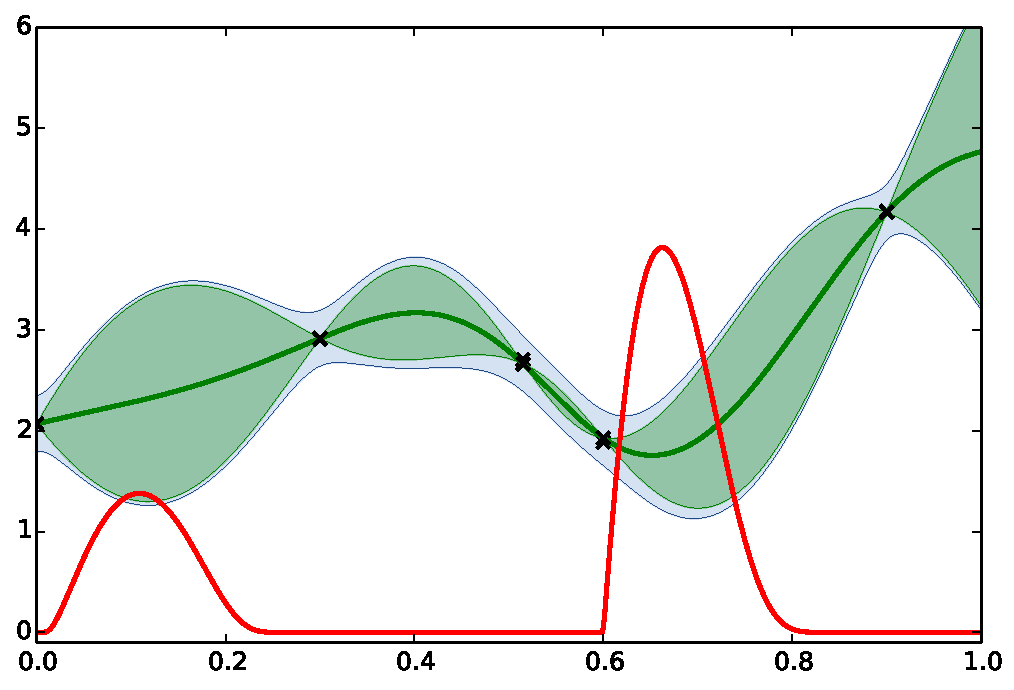
\includegraphics[height=5cm]{4_optimization/figures/python/ego_EI1n0}
\end{center}
\end{frame}

%%%%%%%%%%%%%%%%%%%%%%%%%%%%%%%%%%%%%%%%%%%%%%%%%%%%%%
\begin{frame}[noframenumbering]{Solution 1}
iteration 1
\begin{center}
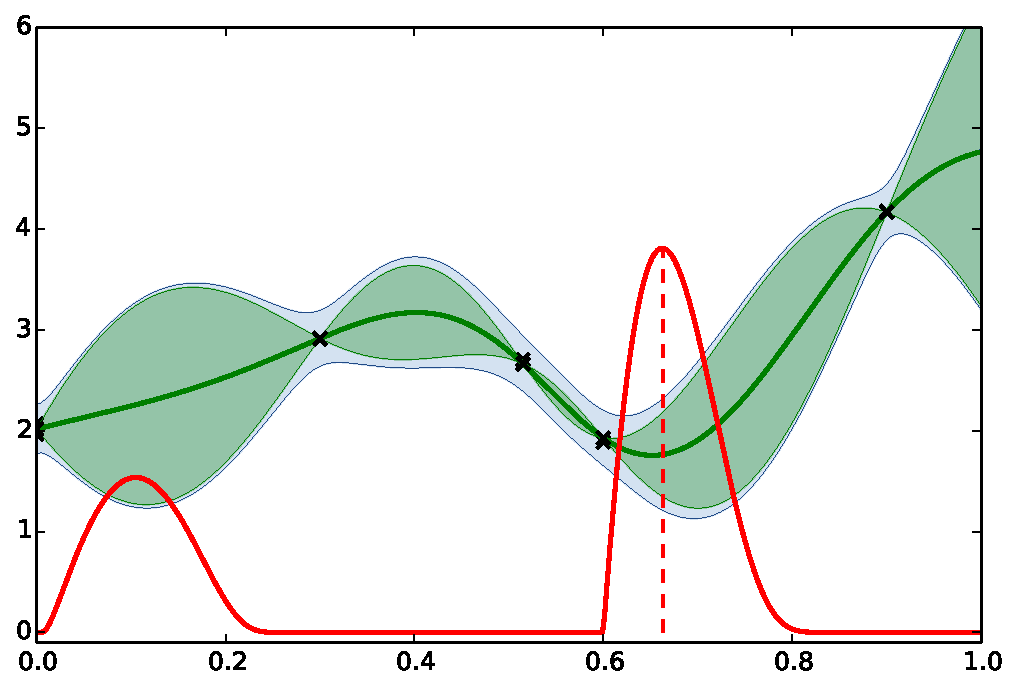
\includegraphics[height=5cm]{4_optimization/figures/python/ego_EI1n1}
\end{center}
\end{frame}

%%%%%%%%%%%%%%%%%%%%%%%%%%%%%%%%%%%%%%%%%%%%%%%%%%%%%%
\begin{frame}[noframenumbering]{Solution 1}
iteration 2
\begin{center}
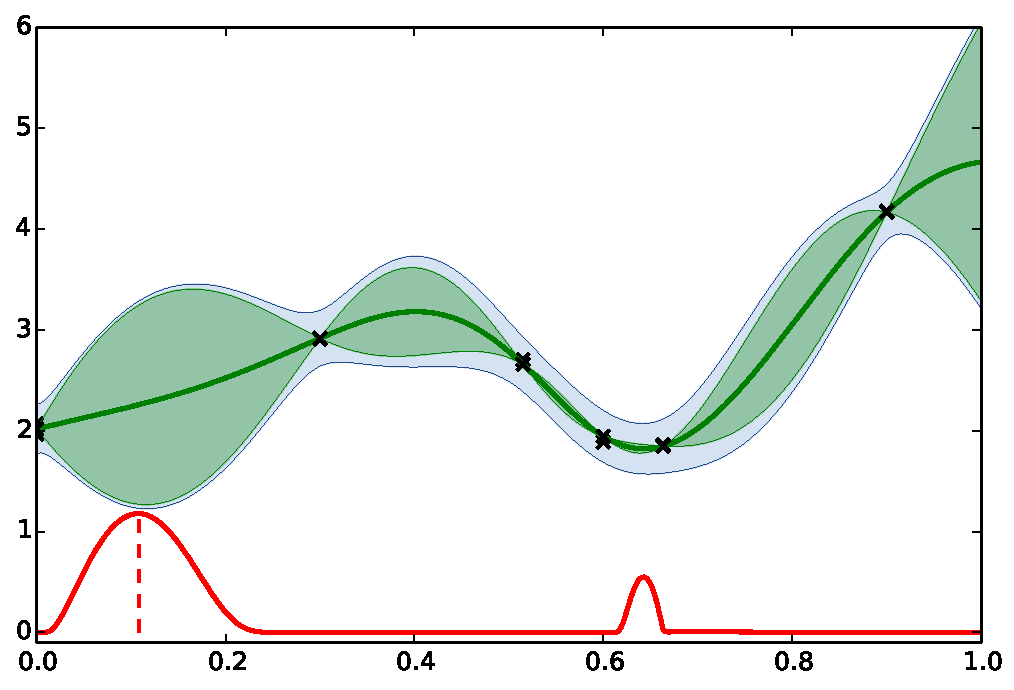
\includegraphics[height=5cm]{4_optimization/figures/python/ego_EI1n2}
\end{center}
\end{frame}

%%%%%%%%%%%%%%%%%%%%%%%%%%%%%%%%%%%%%%%%%%%%%%%%%%%%%%
\begin{frame}[noframenumbering]{Solution 1}
iteration 3
\begin{center}
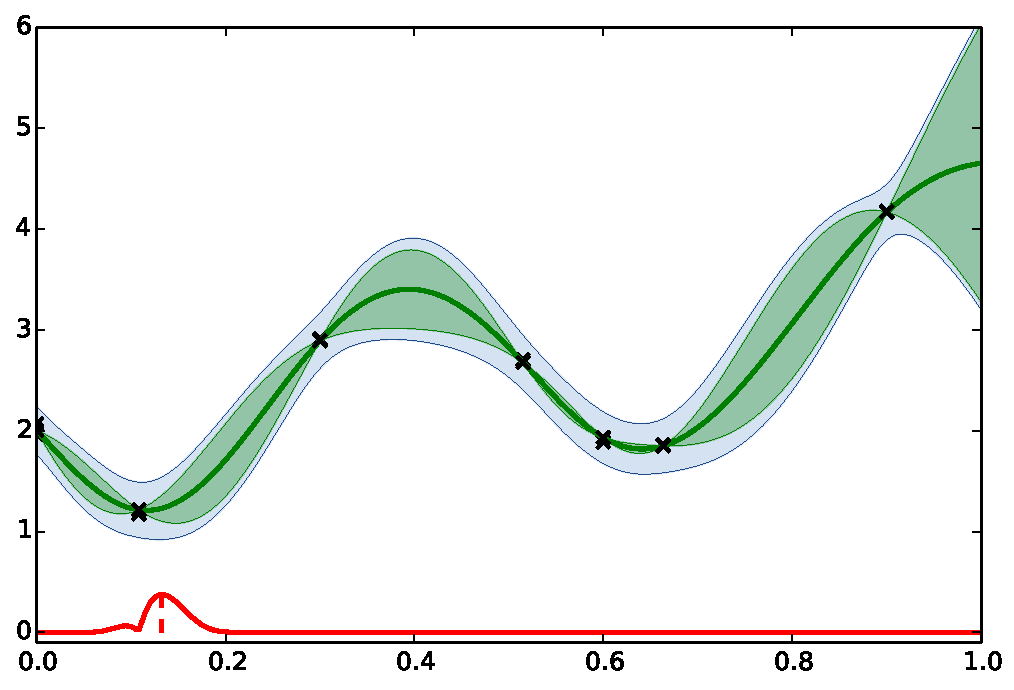
\includegraphics[height=5cm]{4_optimization/figures/python/ego_EI1n3}
\end{center}
\end{frame}

%%%%%%%%%%%%%%%%%%%%%%%%%%%%%%%%%%%%%%%%%%%%%%%%%%%%%%
\begin{frame}[noframenumbering]{Solution 1}
iteration 4
\begin{center}
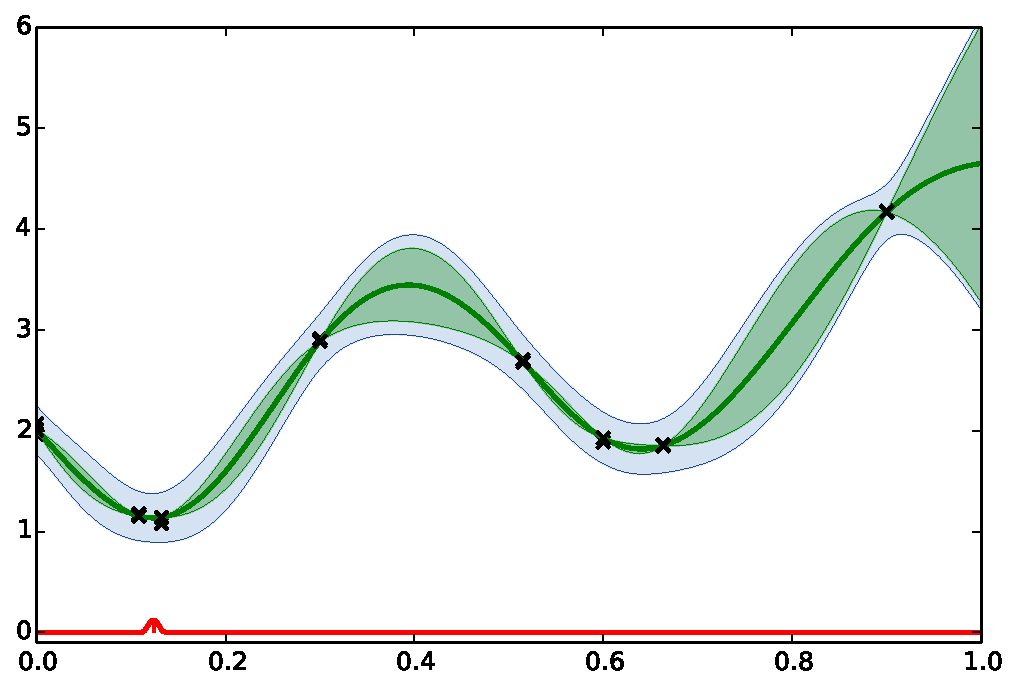
\includegraphics[height=5cm]{4_optimization/figures/python/ego_EI1n4}
\end{center}
\end{frame}

%%%%%%%%%%%%%%%%%%%%%%%%%%%%%%%%%%%%%%%%%%%%%%%%%%%%%%
%%%%%%%%%%%%%%%%%%%%%%%%%%%%%%%%%%%%%%%%%%%%%%%%%%%%%%
\section[Related problems]{Related problems}
\subsection{}

%%%%%%%%%%%%%%%%%%%%%%%%%%%%%%%%%%%%%%%%%%%%%%%%%%%%%%
\begin{frame}{}
Some related optimization problems are:
\begin{itemize}
	\item calibration problems
	\item probability computations
\end{itemize}
\vspace{8mm}
Some algorithms with an EGO spirit can be applied:
\begin{itemize}
 	\item SUR methods
 \end{itemize}
\end{frame}

%%%%%%%%%%%%%%%%%%%%%%%%%%%%%%%%%%%%%%%%%%%%%%%%%%%%%%
\begin{frame}{}
We want to find the input(s) such that f(x) = 3.2
\begin{center}
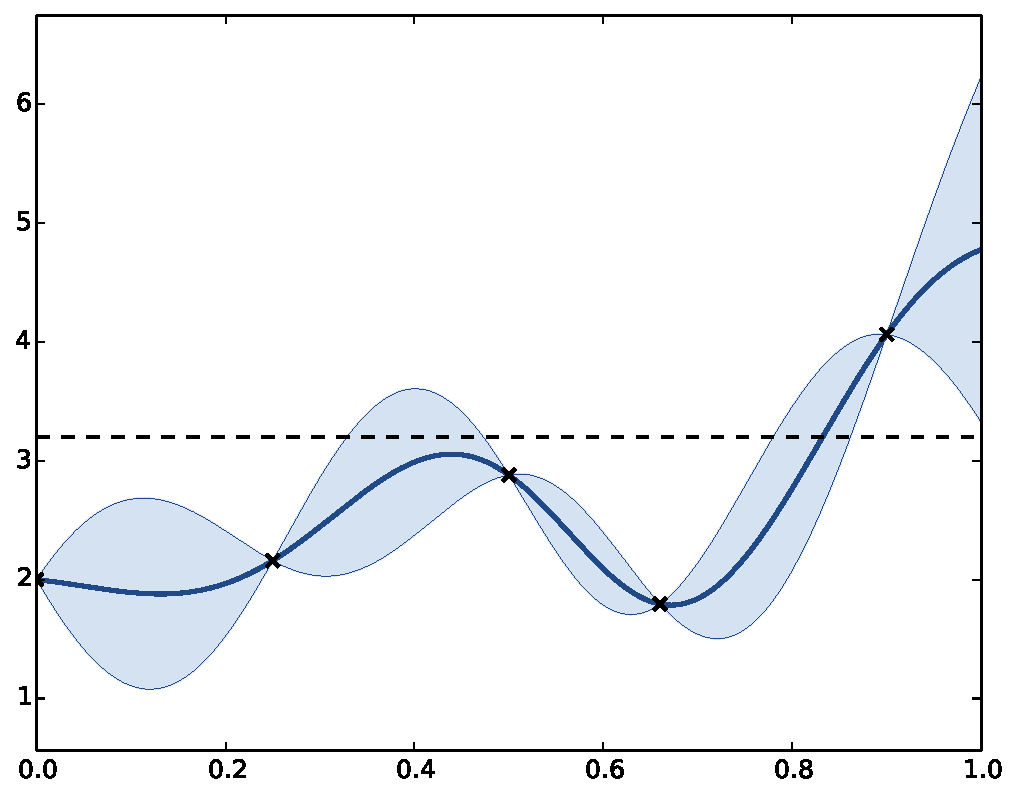
\includegraphics[height=5cm]{4_optimization/figures/python/inv}
\end{center}
\end{frame}

%%%%%%%%%%%%%%%%%%%%%%%%%%%%%%%%%%%%%%%%%%%%%%%%%%%%%%
\begin{frame}[noframenumbering]{}
iteration 0:
\begin{center}
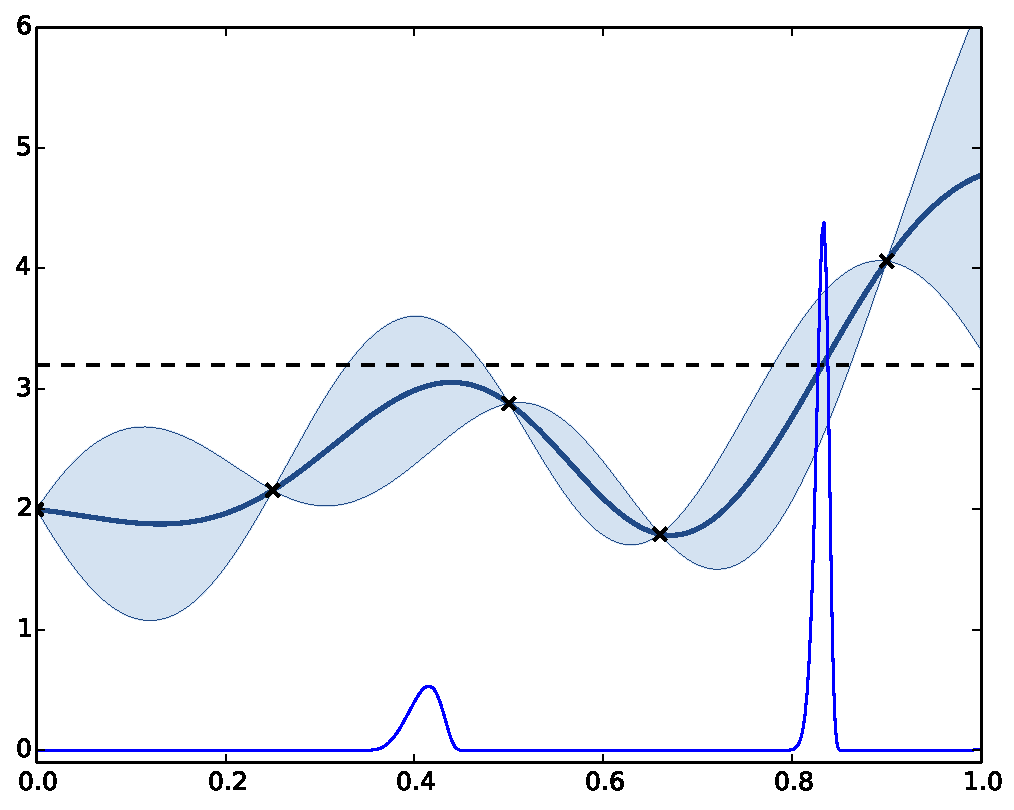
\includegraphics[height=5cm]{4_optimization/figures/python/invproba}
\end{center}
\end{frame}

%%%%%%%%%%%%%%%%%%%%%%%%%%%%%%%%%%%%%%%%%%%%%%%%%%%%%%
\begin{frame}[noframenumbering]{}
iteration 1:
\begin{center}
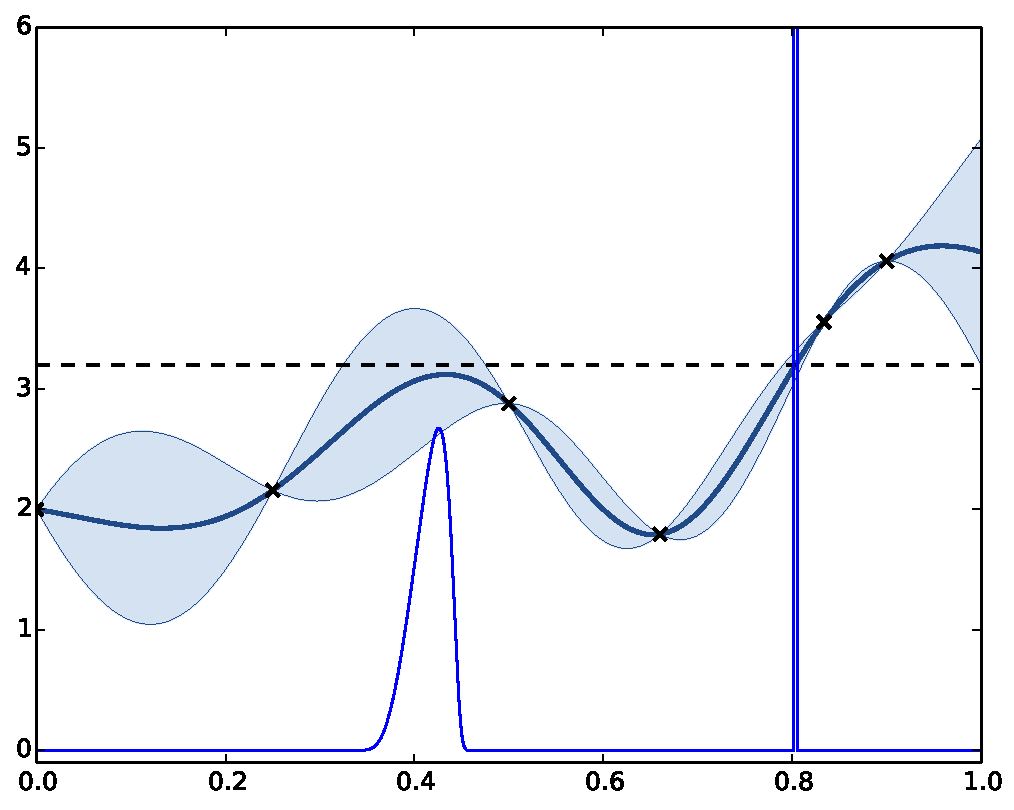
\includegraphics[height=5cm]{4_optimization/figures/python/invproba1}
\end{center}
\end{frame}

%%%%%%%%%%%%%%%%%%%%%%%%%%%%%%%%%%%%%%%%%%%%%%%%%%%%%%
\begin{frame}[noframenumbering]{}
iteration 2:
\begin{center}
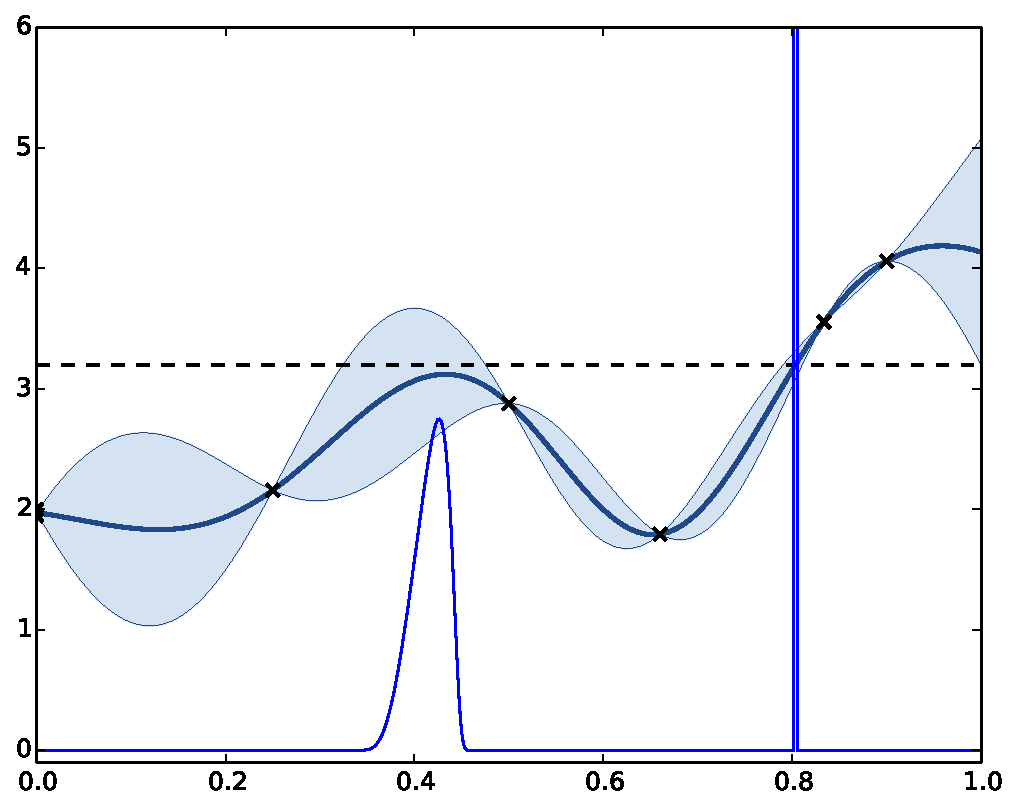
\includegraphics[height=5cm]{4_optimization/figures/python/invproba2}
\end{center}
\end{frame}

%%%%%%%%%%%%%%%%%%%%%%%%%%%%%%%%%%%%%%%%%%%%%%%%%%%%%%
\begin{frame}[noframenumbering]{}
iteration 3:
\begin{center}
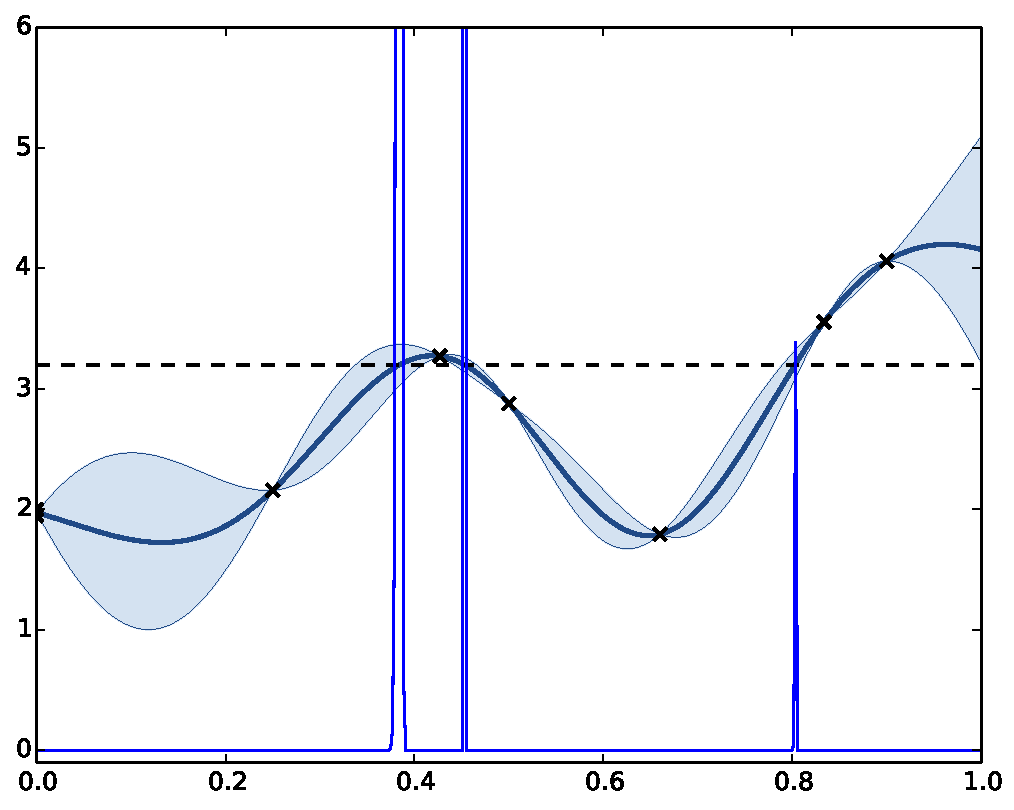
\includegraphics[height=5cm]{4_optimization/figures/python/invproba3}
\end{center}
\end{frame}

